\documentclass[10pt,twocolumn,letterpaper]{article}

% ---------------------------------------------------------------- packages --
\usepackage[T1]{fontenc}
\usepackage[utf8]{inputenc}
\usepackage{mathptmx}
\usepackage[scaled=0.90]{helvet}
\usepackage{courier}
\usepackage{amsmath,amssymb}
\usepackage{graphicx}
\usepackage{booktabs}
\usepackage{array}
\usepackage{multirow}
\usepackage{siunitx}
\usepackage{xcolor}
\usepackage{microtype}
\usepackage{titlesec}
\usepackage{authblk}
\usepackage[font=small,labelfont=bf,labelsep=period]{caption}
\usepackage{subcaption}
\usepackage{enumitem}
\usepackage{stfloats}
\usepackage[hidelinks,breaklinks]{hyperref}
\usepackage[round,authoryear]{natbib}
\usepackage[margin=0.85in,columnsep=0.28in]{geometry}
\usepackage{fancyhdr}
\usepackage[most]{tcolorbox}

% ---------------------------------------------------------------- styling ---
\definecolor{rule}{HTML}{2C4A63}
\definecolor{shade}{HTML}{F0F3F6}
\definecolor{accent}{HTML}{1F6F8B}

\titleformat{\section}{\normalfont\sffamily\bfseries\large\color{rule}}{\thesection}{0.6em}{}
\titleformat{\subsection}{\normalfont\sffamily\bfseries\normalsize\color{rule}}{\thesubsection}{0.6em}{}
\titleformat{\subsubsection}{\normalfont\sffamily\bfseries\small\color{rule}}{\thesubsubsection}{0.6em}{}
\titlespacing*{\section}{0pt}{1.6ex plus .3ex}{0.7ex}
\titlespacing*{\subsection}{0pt}{1.3ex plus .3ex}{0.5ex}

\setlength{\parskip}{0pt}
\renewcommand{\arraystretch}{1.12}
\sisetup{group-separator={,},group-minimum-digits=4,detect-all}

\pagestyle{fancy}
\fancyhf{}
\renewcommand{\headrulewidth}{0.4pt}
\fancyhead[L]{\footnotesize\sffamily\color{rule}Al Fahad --- Probabilistic county-scale outage risk over Michigan}
\fancyfoot[C]{\thepage}
\fancypagestyle{plain}{\fancyhf{}\renewcommand{\headrulewidth}{0pt}\fancyfoot[C]{\thepage}}

\newcommand{\CH}{customer-hours}
\newcommand{\up}{\ensuremath{\uparrow}}
\newcommand{\dn}{\ensuremath{\downarrow}}

% a compact "note" block for the placeholder-economics warning
\newtcolorbox{notebox}{
  colback=shade, colframe=accent, boxrule=0pt, leftrule=2.2pt,
  arc=0pt, outer arc=0pt, left=6pt, right=6pt, top=5pt, bottom=5pt,
  boxsep=0pt, before skip=8pt, after skip=8pt}

% ------------------------------------------------------------------- title --
\title{\vspace{-1.2em}\sffamily\bfseries\Large
Probabilistic County-Scale Prediction of Storm-Driven Power Outages\\[0.15em]
and the Decision Value of Ensemble Forecasts over Michigan}

\author[1]{Abdullah Al Fahad}
\affil[1]{\normalsize NASA Goddard Space Flight Center, Greenbelt, MD, USA}
\date{\normalsize\itshape Preprint --- compiled \today}

\begin{document}

\twocolumn[
\begin{@twocolumnfalse}
\maketitle
\vspace{-2.2em}
\begin{center}
\rule{0.92\textwidth}{0.8pt}
\end{center}
\vspace{-0.6em}

\begin{quote}
\small
\noindent\textbf{Abstract.}
Distribution-system power outages are the weather impact that electricity
customers actually experience, yet operational planning questions --- how much
outage consequence should be expected in each county, and whether a forecast is
good enough to act on --- are seldom answered probabilistically. We present a
reproducible, end-to-end framework that links ERA5 reanalysis and NOAA GEFS
ensemble forecasts to county-day outage records from the EAGLE-I archive across
Michigan for 2018--2023. A three-part hurdle model estimates (i)~the probability
that a county-day experiences an outage event, (ii)~the conditional distribution
of \CH{} lost, and (iii)~the conditional restoration duration under
right-censoring; Monte Carlo composition combines the three into a predictive
distribution of consequence that preserves zero inflation and heavy tails. The
model was frozen on pre-2023 data and scored \emph{once} on the full 2023
holdout. On that holdout the occurrence model attains a Brier score of $0.0795$,
improving on county climatology ($0.0859$), a reduced logistic GLM ($0.0840$),
and a $\SI{20}{\meter\per\second}$ gust-threshold rule ($0.1118$); magnitude
skill relative to climatology remains positive (CRPS skill $+0.084$) and
restoration concordance is $0.619$. Two 2023 GEFS case studies isolate where the
framework is and is not reliable: all four lead times of an August convective
wind event contained the observation within their 10--90\% predictive intervals,
whereas every lead time of a February ice storm fell below it. A cost--loss
analysis translates calibrated probabilities into decision value; at a
cost--loss ratio of $0.10$ and a five-day lead, triggered counties contained
$99\%$ of the realized event loss. The framework is region-portable through a
single configuration file, and all interruption-cost figures are explicitly
flagged as placeholders pending utility-specific inputs.
\end{quote}

\vspace{0.3em}
\noindent\small\textbf{Keywords:} power outage prediction; probabilistic
forecasting; ensemble forecast value; ERA5; GEFS; EAGLE-I; cost--loss analysis;
energy resilience.

\vspace{-0.2em}
\begin{center}
\rule{0.92\textwidth}{0.8pt}
\end{center}
\vspace{1.0em}
\end{@twocolumnfalse}
]

% ============================================================================
\section{Introduction}
% ============================================================================

Severe weather is the dominant cause of sustained interruptions on electricity
distribution systems, and the consequence borne by customers is measured not in
damaged assets but in service lost. Utilities and emergency managers therefore
face a forecasting problem that is only partly meteorological: given the
atmospheric state expected over a region, how much outage consequence should be
anticipated, where, and is the anticipated consequence large enough and certain
enough to justify pre-positioning crews, requesting mutual aid, or issuing
public advisories?

A substantial literature addresses the first half of this
question. Statistical outage-prediction models have been developed for tropical
cyclones \citep{guikema2014hurricane,nateghi2014outage} and for extratropical
storms in the northeastern United States
\citep{wanik2015storm,cerrai2019outages}, generally by regressing outage counts
on hazard, land-cover, and network covariates. These studies established that
weather-conditioned statistical models can substantially outperform
climatological and threshold baselines. Two features of the operational problem
have received less attention. First, most published models target a conditional
\emph{mean} or a deterministic count, whereas the quantity a planner needs is a
full predictive \emph{distribution}: outage consequence is zero-inflated and
heavy-tailed, and the decision-relevant information sits in the upper tail.
Second, statistical skill is usually reported without translating it into
decision value, so it remains unclear whether a given level of skill would have
changed any action.

This paper addresses both. We construct a county-day probabilistic model of
outage consequence for Michigan over 2018--2023 and evaluate it under a strictly
frozen experimental design, then carry the calibrated probabilities through a
cost--loss decision framework \citep{richardson2000value,zhu2002economicvalue}
to quantify the operational value of acting on them.

Three design commitments shape what follows.

\begin{description}[leftmargin=1.1em,itemsep=0.25em,topsep=0.3em]
\item[\textnormal{\emph{Consequence, not fragility.}}] The target is what
customers experienced --- probability of an outage event, \CH{} lost, and
restoration duration --- and not the physical failure of any asset. County-level
outage records contain no information about which pole or conductor failed, and
we make no claim about physical damage.

\item[\textnormal{\emph{Distributions, not point forecasts.}}] Every stage emits
a predictive distribution, and every headline metric is a proper scoring rule
\citep{gneiting2007scoringrules} or a calibration diagnostic
\citep{gneiting2007calibration}, evaluated against explicitly stated reference
forecasts.

\item[\textnormal{\emph{One test, scored once.}}] The temporal split was fixed
before the data were examined. The 2023 holdout was opened a single time, after
the model, the calibrator, the reporting cohort, and the configuration hash were
frozen. No 2023 outcome informed tuning, calibration, bias correction, or model
selection.
\end{description}

Section~\ref{sec:data} describes the inputs; Section~\ref{sec:methods} the model
and verification framework; Section~\ref{sec:results} the frozen-model results;
Section~\ref{sec:value} the decision-value analysis; and
Section~\ref{sec:discussion} what the results do and do not support.

% ============================================================================
\section{Data}\label{sec:data}
% ============================================================================

\subsection{Outage observations}

Outage consequence is derived from the EAGLE-I archive of recorded county-level
electricity outages \citep{brelsford2024eaglei}, which reports the number of
customers without service by county at approximately 15-minute resolution.
Records are resampled to hourly county series and normalized by Monthly County
Customer (MCC) counts to give an outage fraction $f_{ct}$ for county $c$ at hour
$t$.

Two properties of this archive drive the preprocessing. Reporting coverage is
not uniform across counties or years, so the study defines a \emph{frozen
reporting cohort}: counties with stable annual coverage across the training and
validation years. Counties whose coverage changes within that window are
excluded, and any coverage gap confined to the test year is recorded as a stated
limitation rather than used to alter the cohort --- changing the study population
between fitting and testing would make the holdout something other than a
held-out test. Second, a nonzero baseline of routine, non-storm outages is
always present. We remove it with a rolling 30-day 10th-percentile baseline per
county and work with the excess fraction
$f^{\mathrm{exc}}_{ct}=\max(f_{ct}-b_{ct},0)$.

\subsection{Event definition}

An \emph{outage event} begins when $f^{\mathrm{exc}}_{ct}$ exceeds
$0.5\%$ of county customers, must persist at least $2$ hours, and merges with a
neighbouring exceedance separated by less than $6$ hours. Restoration is
declared when the excess fraction decays to $10\%$ of the event peak. Events
still active at the end of the record are marked right-censored and treated as
such by the duration model. For each county-day the event table yields the
binary occurrence indicator $Y_{ct}$, the integrated consequence in \CH{}, the
peak outage fraction, the restoration duration, and a concurrent statewide load
term.

\subsection{Atmospheric predictors}

Hourly ERA5 reanalysis \citep{hersbach2020era5} supplies 10\,m and 100\,m winds,
instantaneous 10\,m wind gust, total precipitation, 2\,m temperature,
volumetric soil water in the upper two layers, convective available potential
energy, snowfall, and snow depth over a Michigan domain. Forecast case studies
use the NOAA Global Ensemble Forecast System version~12
\citep{zhou2022gefsv12}, 31 members at $0.25^\circ$, at lead times of
$5$, $3$, $2$, and $1$ days.

\subsection{Static exposure}

County geometry comes from U.S.\ Census TIGER/Line. NLCD percent tree canopy
cover \citep{coulston2012tcc} provides a county-mean vegetation exposure proxy.
We stress that canopy cover is an exposure proxy only: it carries no information
about vegetation-management practice, trim cycles, or right-of-way condition,
which are among the strongest real controls on storm outage rates and are not
observable in any public dataset used here.

% ============================================================================
\section{Methods}\label{sec:methods}
% ============================================================================

\begin{figure*}[!tb]
\centering
\includegraphics[width=0.94\textwidth]{../figures/storm_outage_workflow.pdf}
\caption{Analysis workflow. Hourly ERA5 reanalysis, EAGLE-I county outage
records, NLCD canopy, and GEFS ensemble forecasts are aggregated to county-day
features in an equal-area projection; a three-part probabilistic model produces
county-day risk, and Monte Carlo composition supplies the predictive
distributions used in the decision-value analysis. The maps, curves, and density
shapes in this schematic illustrate the analysis design; empirical results
appear in Section~\ref{sec:results}.}
\label{fig:workflow}
\end{figure*}

Figure~\ref{fig:workflow} summarizes the pipeline. Each stage is described
below.

\subsection{Spatial aggregation and county-day features}

The ERA5 $0.25^\circ$ grid is aggregated to county polygons in the CONUS Albers
equal-area projection (EPSG:5070). Two aggregation operators are maintained
rather than one, because the correct operator depends on the physics of the
field. Smooth fields --- temperature, soil moisture, accumulated precipitation ---
are aggregated with area weights that sum to unity per county. Localized damage
agents --- wind gust and CAPE --- are aggregated with spatial maxima and upper
percentiles over the cells intersecting each county. Using an area-weighted mean
for gust is not a conservative choice but a destructive one: it averages the
peak gust of a squall line together with calm cells at the far end of the county
and removes precisely the signal that damages the network.

Hourly county series are then reduced to daily features: maximum and
95th-percentile gust, mean gust, maximum sustained and 100\,m winds, total and
maximum hourly precipitation, hours above gust thresholds of $13$, $18$, and
$\SI{25}{\meter\per\second}$, mean soil moisture, maximum CAPE, minimum and
maximum temperature, a freezing-rain proxy (precipitation accumulated while 2\,m
temperature lies in $[-2,+0.5]\,^\circ$C), a wet-snow proxy (snowfall
accumulated while temperature lies in $[-1,+1]\,^\circ$C), 7-day antecedent
precipitation, and interaction terms coupling gust to canopy, soil moisture, and
a leaf-on indicator. A heuristic regime label (convective wind, synoptic wind,
ice, wet snow, benign) is attached for stratified verification; it is a
diagnostic convenience, not ground truth.

\subsection{Three-part probabilistic model}

For county $c$ and day $t$ the model estimates a predictive distribution of
consequence, decomposed as a hurdle:

\begin{equation}
p_{ct} = P\!\left(Y_{ct}=1 \mid \mathbf{X}_{ct}\right),
\label{eq:occ}
\end{equation}

\noindent estimated by gradient-boosted decision trees
\citep{friedman2001gbm,ke2017lightgbm} under a binary objective with
positive-class reweighting, then mapped to calibrated probabilities by isotonic
regression \citep{zadrozny2002calibration} fitted on the validation window;

\begin{equation}
H_{ct} \mid Y_{ct}=1 \;\sim\; F_{\mathbf{X}_{ct}},
\label{eq:mag}
\end{equation}

\noindent the conditional distribution of \CH{}, estimated in $\log(1+\cdot)$
space by natural-gradient boosting of a Gaussian density
\citep{duan2020ngboost}, with independently fitted pinball-loss quantile models
as a documented fallback; and

\begin{equation}
T_{ct} \mid Y_{ct}=1 \;\sim\; \mathrm{Weibull\ AFT}(\mathbf{X}_{ct}),
\label{eq:dur}
\end{equation}

\noindent the conditional restoration duration, fitted as an accelerated failure
time model that treats unresolved events as right-censored
\citep{kalbfleisch2002failuretime}, with a Cox proportional-hazards fit retained
as a diagnostic.

Reported quantiles are $\{0.05,0.10,0.25,0.50,0.75,0.90,0.95\}$. Where
independently fitted quantile regressions cross, monotonicity is restored by
rearrangement, and the raw crossing count is recorded as evidence about how hard
the quantile route is straining.

\subsection{Monte Carlo composition}

The three stages are composed by Monte Carlo: for each county-day, $1000$ draws
sample occurrence from~\eqref{eq:occ}, and for the draws that fire, magnitude
from~\eqref{eq:mag} and duration from~\eqref{eq:dur}. Composition rather than
multiplication of conditional means is what preserves the zero inflation and the
heavy right tail; a composed median is not the median of the composition, and
the difference is largest exactly where the decision matters.

\subsection{Verification framework}

Absolute scores are uninformative without reference forecasts, so every
occurrence metric is reported against three: \emph{county} climatology (the
county's own historical event rate), a reduced-feature logistic GLM, and a
$\SI{20}{\meter\per\second}$ gust-threshold rule. County climatology, not a
single statewide rate, is the correct reference: Michigan county event rates
vary by an order of magnitude, and skill measured against a pooled rate flatters
the model. Magnitude is referenced to the training climatological quantiles of
\CH{}, and restoration to county-specific persistence (the county's historical
median restoration time).

Occurrence is scored with the Brier score \citep{brier1950verification} and its
skill relative to county climatology, average precision, ROC AUC, and log loss.
Magnitude is scored with the continuous ranked probability score
\citep{gneiting2007scoringrules}, computed as the pinball-loss integral over a
999-point probability grid with probit-slope tail extrapolation --- not as a
truncated ensemble approximation, which discards the outer predictive mass where
most \CH{} live --- together with a logarithmic score and a probability integral
transform histogram \citep{gneiting2007calibration}. Restoration is scored with
Harrell's concordance index \citep{harrell1982yield} and median absolute error
on uncensored events.

Reported validation probabilities are \emph{out-of-fold} within the validation
window. Isotonic regression is flexible, and scoring a calibrator on the rows it
was fitted on makes every occurrence metric and every reliability diagram look
better than the model is; the in-sample value is retained alongside so the
optimism remains visible rather than being reported as the result.

\subsection{Cross-validation and leakage control}

Adjacent county-days within one storm are not independent observations. Random
folds place the same storm on both sides of a split and reward memorising
storms. We therefore block cross-validation by \emph{storm episode}: a storm day
is one on which at least $10\%$ of reporting counties are in event, consecutive
storm days are merged across gaps of up to two days, and each day is assigned to
its nearest episode. Defining a storm day as one on which \emph{any} county is
in event does not work at this cohort size --- with a per-county event rate of a
few percent, almost every calendar day qualifies and the entire multi-year
record fuses into a single group. Leave-one-county-out and forward-year folds
are retained alongside storm blocking as complementary diagnostics of spatial
and temporal generalization.

\subsection{Experimental design}

\begin{table}[!t]
\centering
\caption{Frozen temporal design. The split was fixed before the data were
examined and was not revisited.}
\label{tab:design}
\small
\begin{tabular}{@{}lll@{}}
\toprule
\textbf{Period} & \textbf{Dates} & \textbf{Role} \\
\midrule
Training    & 2018-01-01 -- 2022-06-30 & Fit the model \\
Validation  & 2022-07-01 -- 2022-12-31 & Calibrate and verify \\
Test        & 2023-01-01 -- 2023-12-31 & One-time evaluation \\
\bottomrule
\end{tabular}
\end{table}

Table~\ref{tab:design} gives the frozen split. All timestamps are UTC. The
fitted model, the isotonic calibrator, the reporting cohort, and a SHA-256 hash
of the full configuration are serialized together; the test evaluation refuses
to run if the configuration hash has changed or if the rebuilt test-year cohort
differs from the frozen one. A marker file records that the test year has been
opened, and is written only after scoring has succeeded.

An earlier January--May 2021 retrospective is superseded and not reported here,
because 2021 is now training data; forward-year cross-validation is the
appropriate temporal diagnostic in the final design.

% ============================================================================
\section{Results}\label{sec:results}
% ============================================================================

\begin{table*}[!tb]
\centering
\caption{Verification of the frozen model. The 2023 column is the primary
result and was produced once, after freezing; validation is shown for context.
Arrows give the direction of improvement. Reference rows are alternative
forecasts, not model outputs.}
\label{tab:verification}
\small
\begin{tabular*}{\textwidth}{@{\extracolsep{\fill}}llrr@{}}
\toprule
\textbf{Metric} & \textbf{Better} & \textbf{Validation} & \textbf{2023 test} \\
\midrule
\multicolumn{4}{@{}l}{\textit{Occurrence}}\\
\quad Brier score                          & \dn & 0.0926 & \textbf{0.0795} \\
\quad Brier skill vs.\ county climatology  & \up & $+0.101$ & $\mathbf{+0.075}$ \\
\quad Average precision                    & \up & 0.339 & \textbf{0.277} \\
\quad ROC AUC                              & \up & 0.753 & \textbf{0.746} \\
\quad Log loss                             & \dn & 0.3196 & \textbf{0.2838} \\
\quad \textit{Ref.}: logistic GLM (Brier)  & \dn & 0.0999 & \textbf{0.0840} \\
\quad \textit{Ref.}: county climatology (Brier) & \dn & 0.1030 & \textbf{0.0859} \\
\quad \textit{Ref.}: gust $>\SI{20}{\meter\per\second}$ rule (Brier) & \dn & 0.1418 & \textbf{0.1118} \\
\addlinespace
\multicolumn{4}{@{}l}{\textit{Magnitude (\CH{} given an event)}}\\
\quad CRPS                                 & \dn & \num{16011} & \textbf{\num{39164}} \\
\quad CRPS skill vs.\ climatology          & \up & $+0.083$ & $\mathbf{+0.084}$ \\
\quad Logarithmic score                    & \dn & 9.242 & \textbf{9.003} \\
\quad Median RMSE                          & \dn & \num{146422} & \textbf{\num{501575}} \\
\addlinespace
\multicolumn{4}{@{}l}{\textit{Restoration duration}}\\
\quad Concordance index                    & \up & 0.663 & \textbf{0.619} \\
\quad Median absolute error (h)            & \dn & 4.42 & \textbf{5.22} \\
\quad \textit{Ref.}: county persistence MAE (h) & \dn & 4.57 & \textbf{4.20} \\
\bottomrule
\end{tabular*}
\end{table*}

\subsection{Occurrence}

On the 2023 holdout the occurrence model attains a Brier score of $0.0795$
(Table~\ref{tab:verification}), improving on all three references: county
climatology ($0.0859$), the reduced logistic GLM ($0.0840$), and the gust
threshold rule ($0.1118$). The Brier skill score against county climatology is
$+0.075$, down from $+0.101$ in validation. Discrimination is stable across the
two windows --- ROC AUC $0.746$ on test against $0.753$ on validation --- while
average precision falls from $0.339$ to $0.277$.

The pattern is worth stating plainly, because the absolute Brier score
\emph{improved} from validation to test while the skill score \emph{declined}.
Both are correct and neither is the headline on its own: 2023 was an easier year
to forecast in absolute terms, and the climatological reference improved along
with the model. Skill relative to climatology is the quantity that generalizes,
and it remained positive but smaller. That the margin over a nine-feature
logistic GLM is modest ($0.0795$ versus $0.0840$) is itself a result: on this
target, most of the achievable occurrence skill is captured by a small set of
interpretable hazard and exposure predictors, and the gradient-boosted model
adds a real but incremental improvement.

Figure~\ref{fig:skill} collects the reliability curve, precision--recall curve,
magnitude PIT histogram, reference-model comparison, regime stratification, and
cross-validation summary for the frozen model.

\begin{figure*}[!tb]
\centering
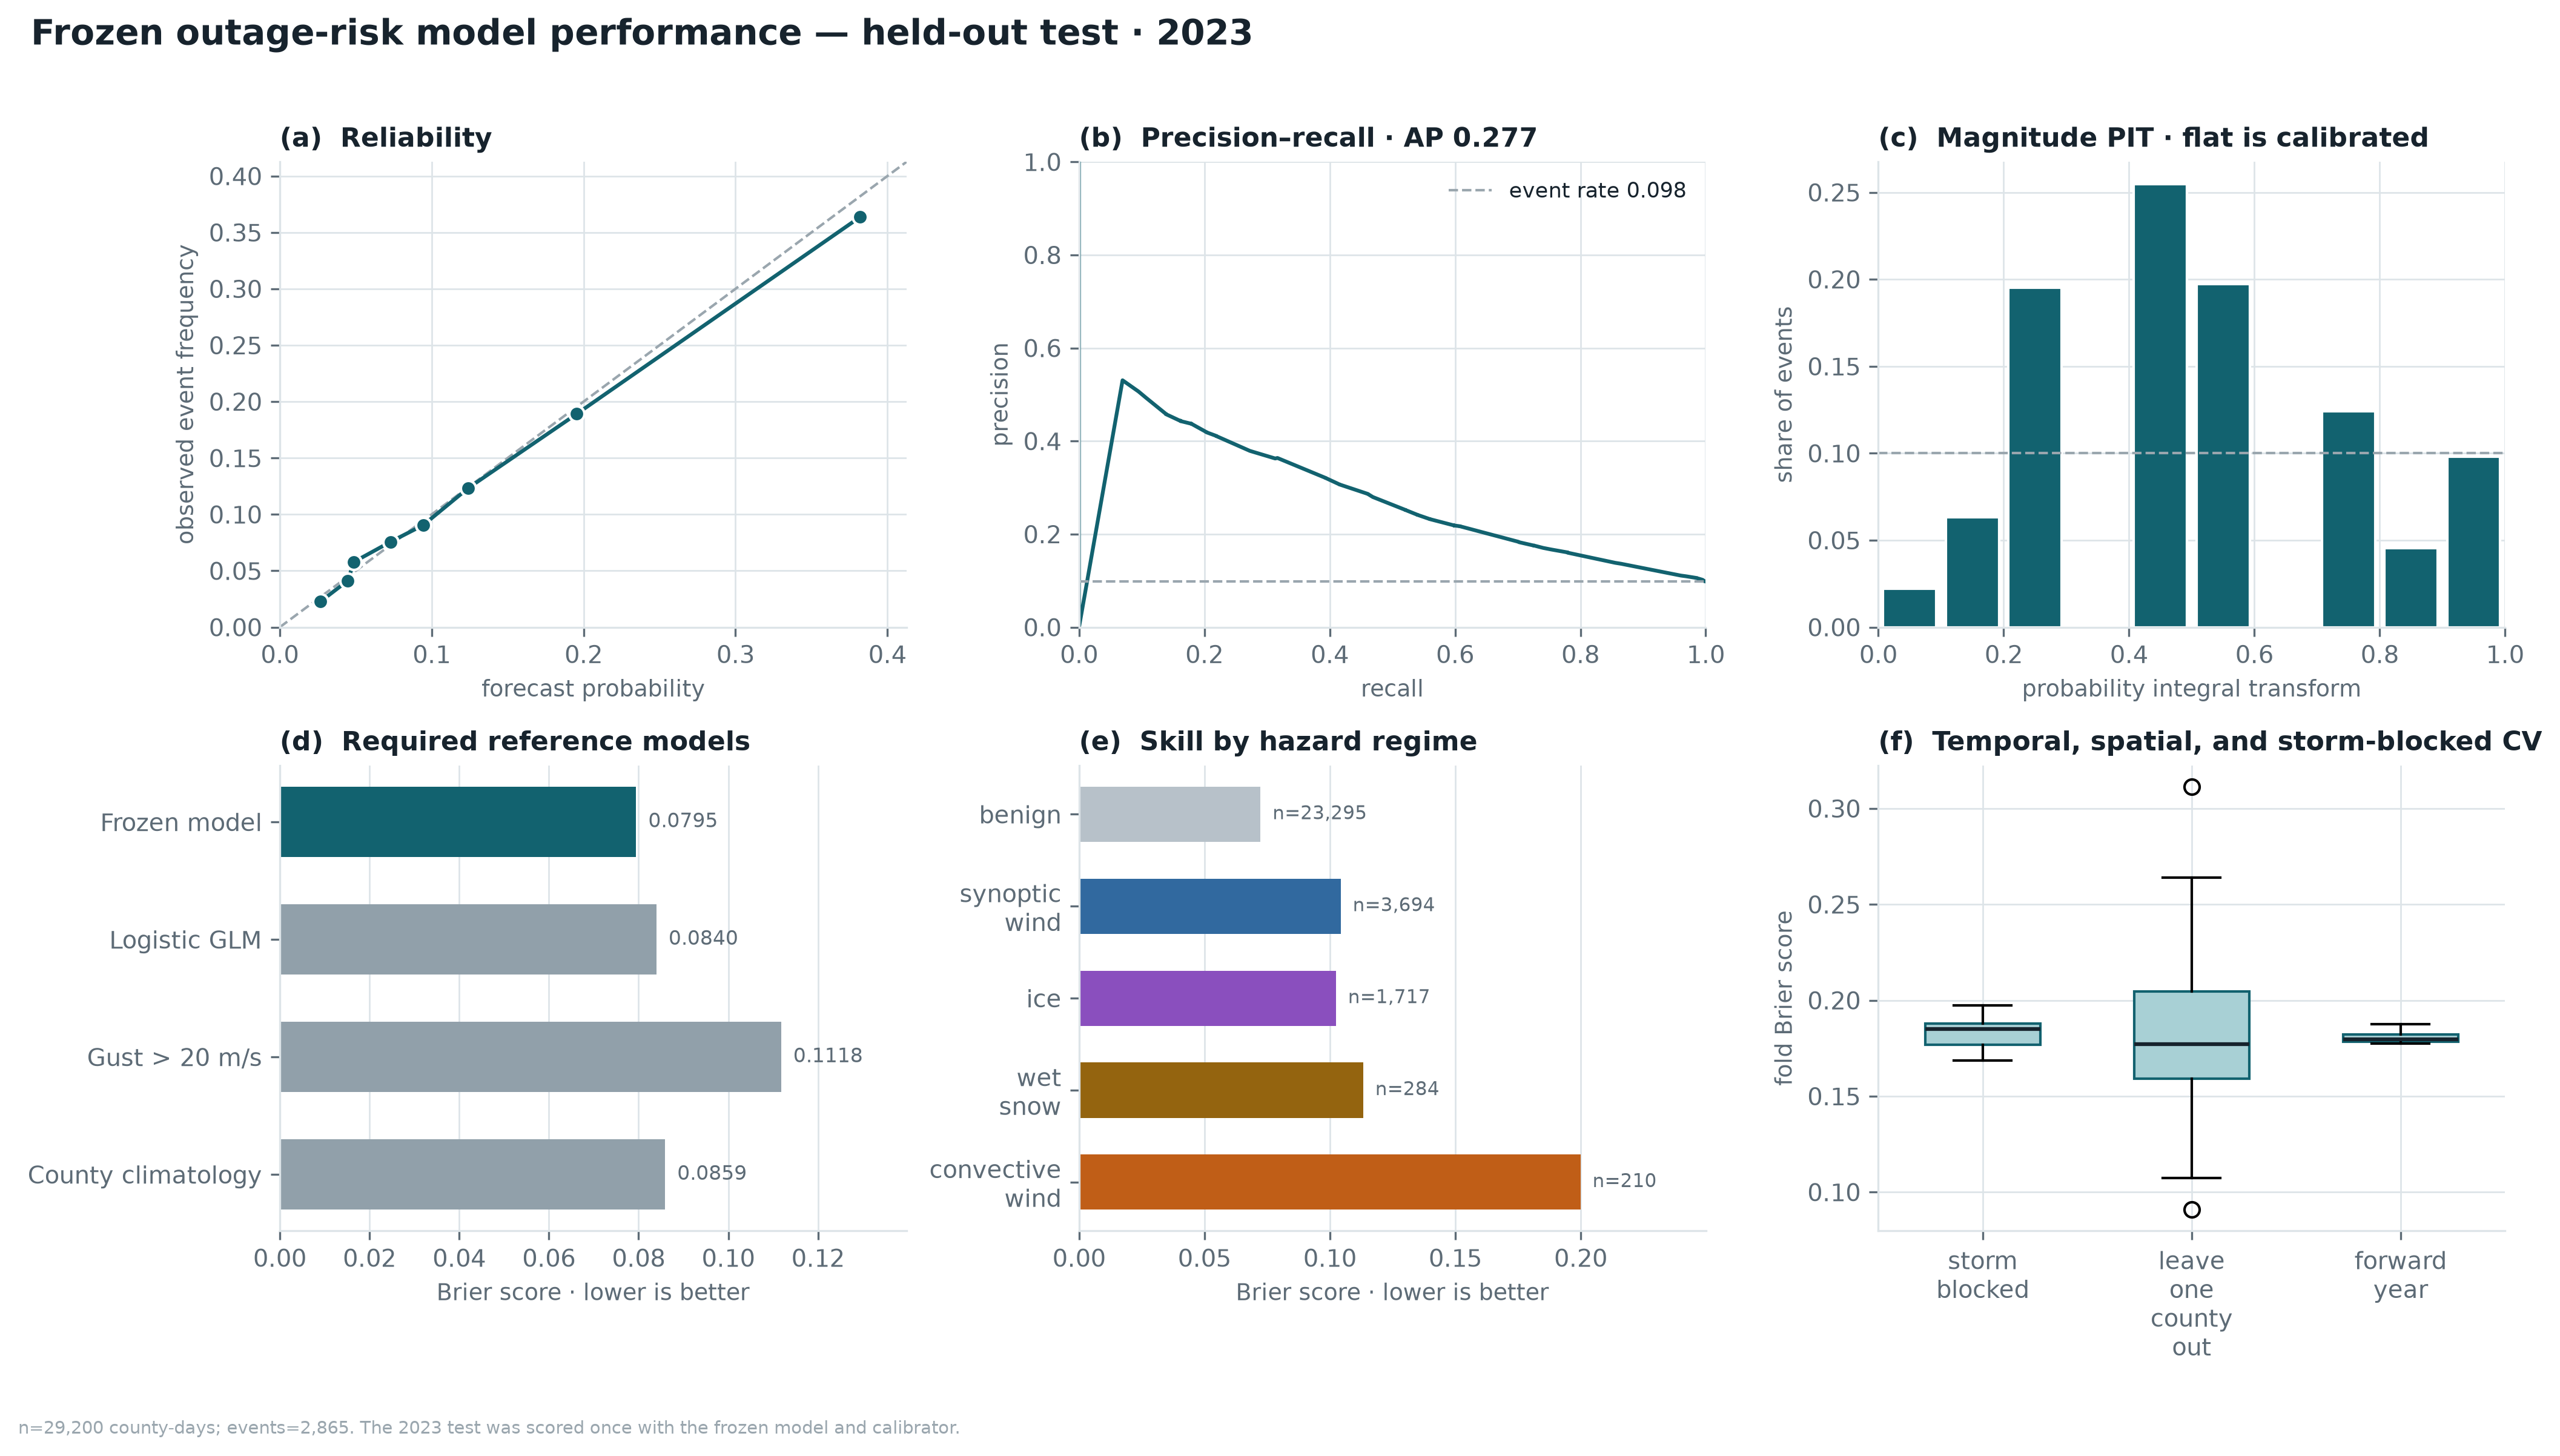
\includegraphics[width=0.95\textwidth]{../figures/phase2_skill_summary.png}
\caption{Frozen-model skill summary: occurrence reliability and
precision--recall, magnitude probability integral transform histogram,
comparison against reference forecasts, stratification by hazard regime, and
cross-validation across storm-blocked, leave-one-county-out, and forward-year
schemes. Reliability uses out-of-fold calibrated probabilities.}
\label{fig:skill}
\end{figure*}

\subsection{Magnitude and restoration}

Magnitude skill relative to the climatological quantiles of \CH{} is
essentially unchanged between windows ($+0.083$ validation, $+0.084$ test), but
the absolute errors are not: CRPS rises from $\num{16011}$ to $\num{39164}$ and
median RMSE from $\num{146422}$ to $\num{501575}$ \CH{}. The stability of the
skill score alongside a threefold rise in absolute error indicates that 2023
contained larger events than the validation half-year rather than that the
magnitude model degraded; the climatological reference deteriorated by a
comparable factor. The very large median RMSE relative to CRPS is the expected
signature of a heavy-tailed target: a proper score integrated over the full
predictive distribution is far more forgiving of tail events than a squared
error on a central estimate, which is one reason CRPS rather than RMSE is the
headline magnitude metric here.

Restoration concordance falls from $0.663$ to $0.619$, and median absolute error
rises from $4.42$ to $5.22$ hours. Notably, the county-persistence reference
achieved $4.20$ hours on the test year --- \emph{better} than the model's
$5.22$. We report this without softening it: on the 2023 holdout, the
restoration model did not beat a county-median persistence baseline on median
absolute error, even though it ranked events better than chance
(concordance $0.619$). Restoration duration is driven by crew dispatch, mutual
aid, and access constraints that no atmospheric predictor observes, and this
result is the clearest quantitative evidence in the study for where utility
operational data would add the most.

\subsection{Spatial diagnostics}

Figure~\ref{fig:county} maps county-level event rate, mean forecast probability,
bias, Brier skill, event count, and magnitude CRPS. Skill is not spatially
uniform, and the counties where it is weakest are informative: sparse-coverage
and low-event-count counties provide few events to learn from, so their
county-specific climatology is itself poorly estimated and the skill score
against it is correspondingly noisy.

\begin{figure*}[!tb]
\centering
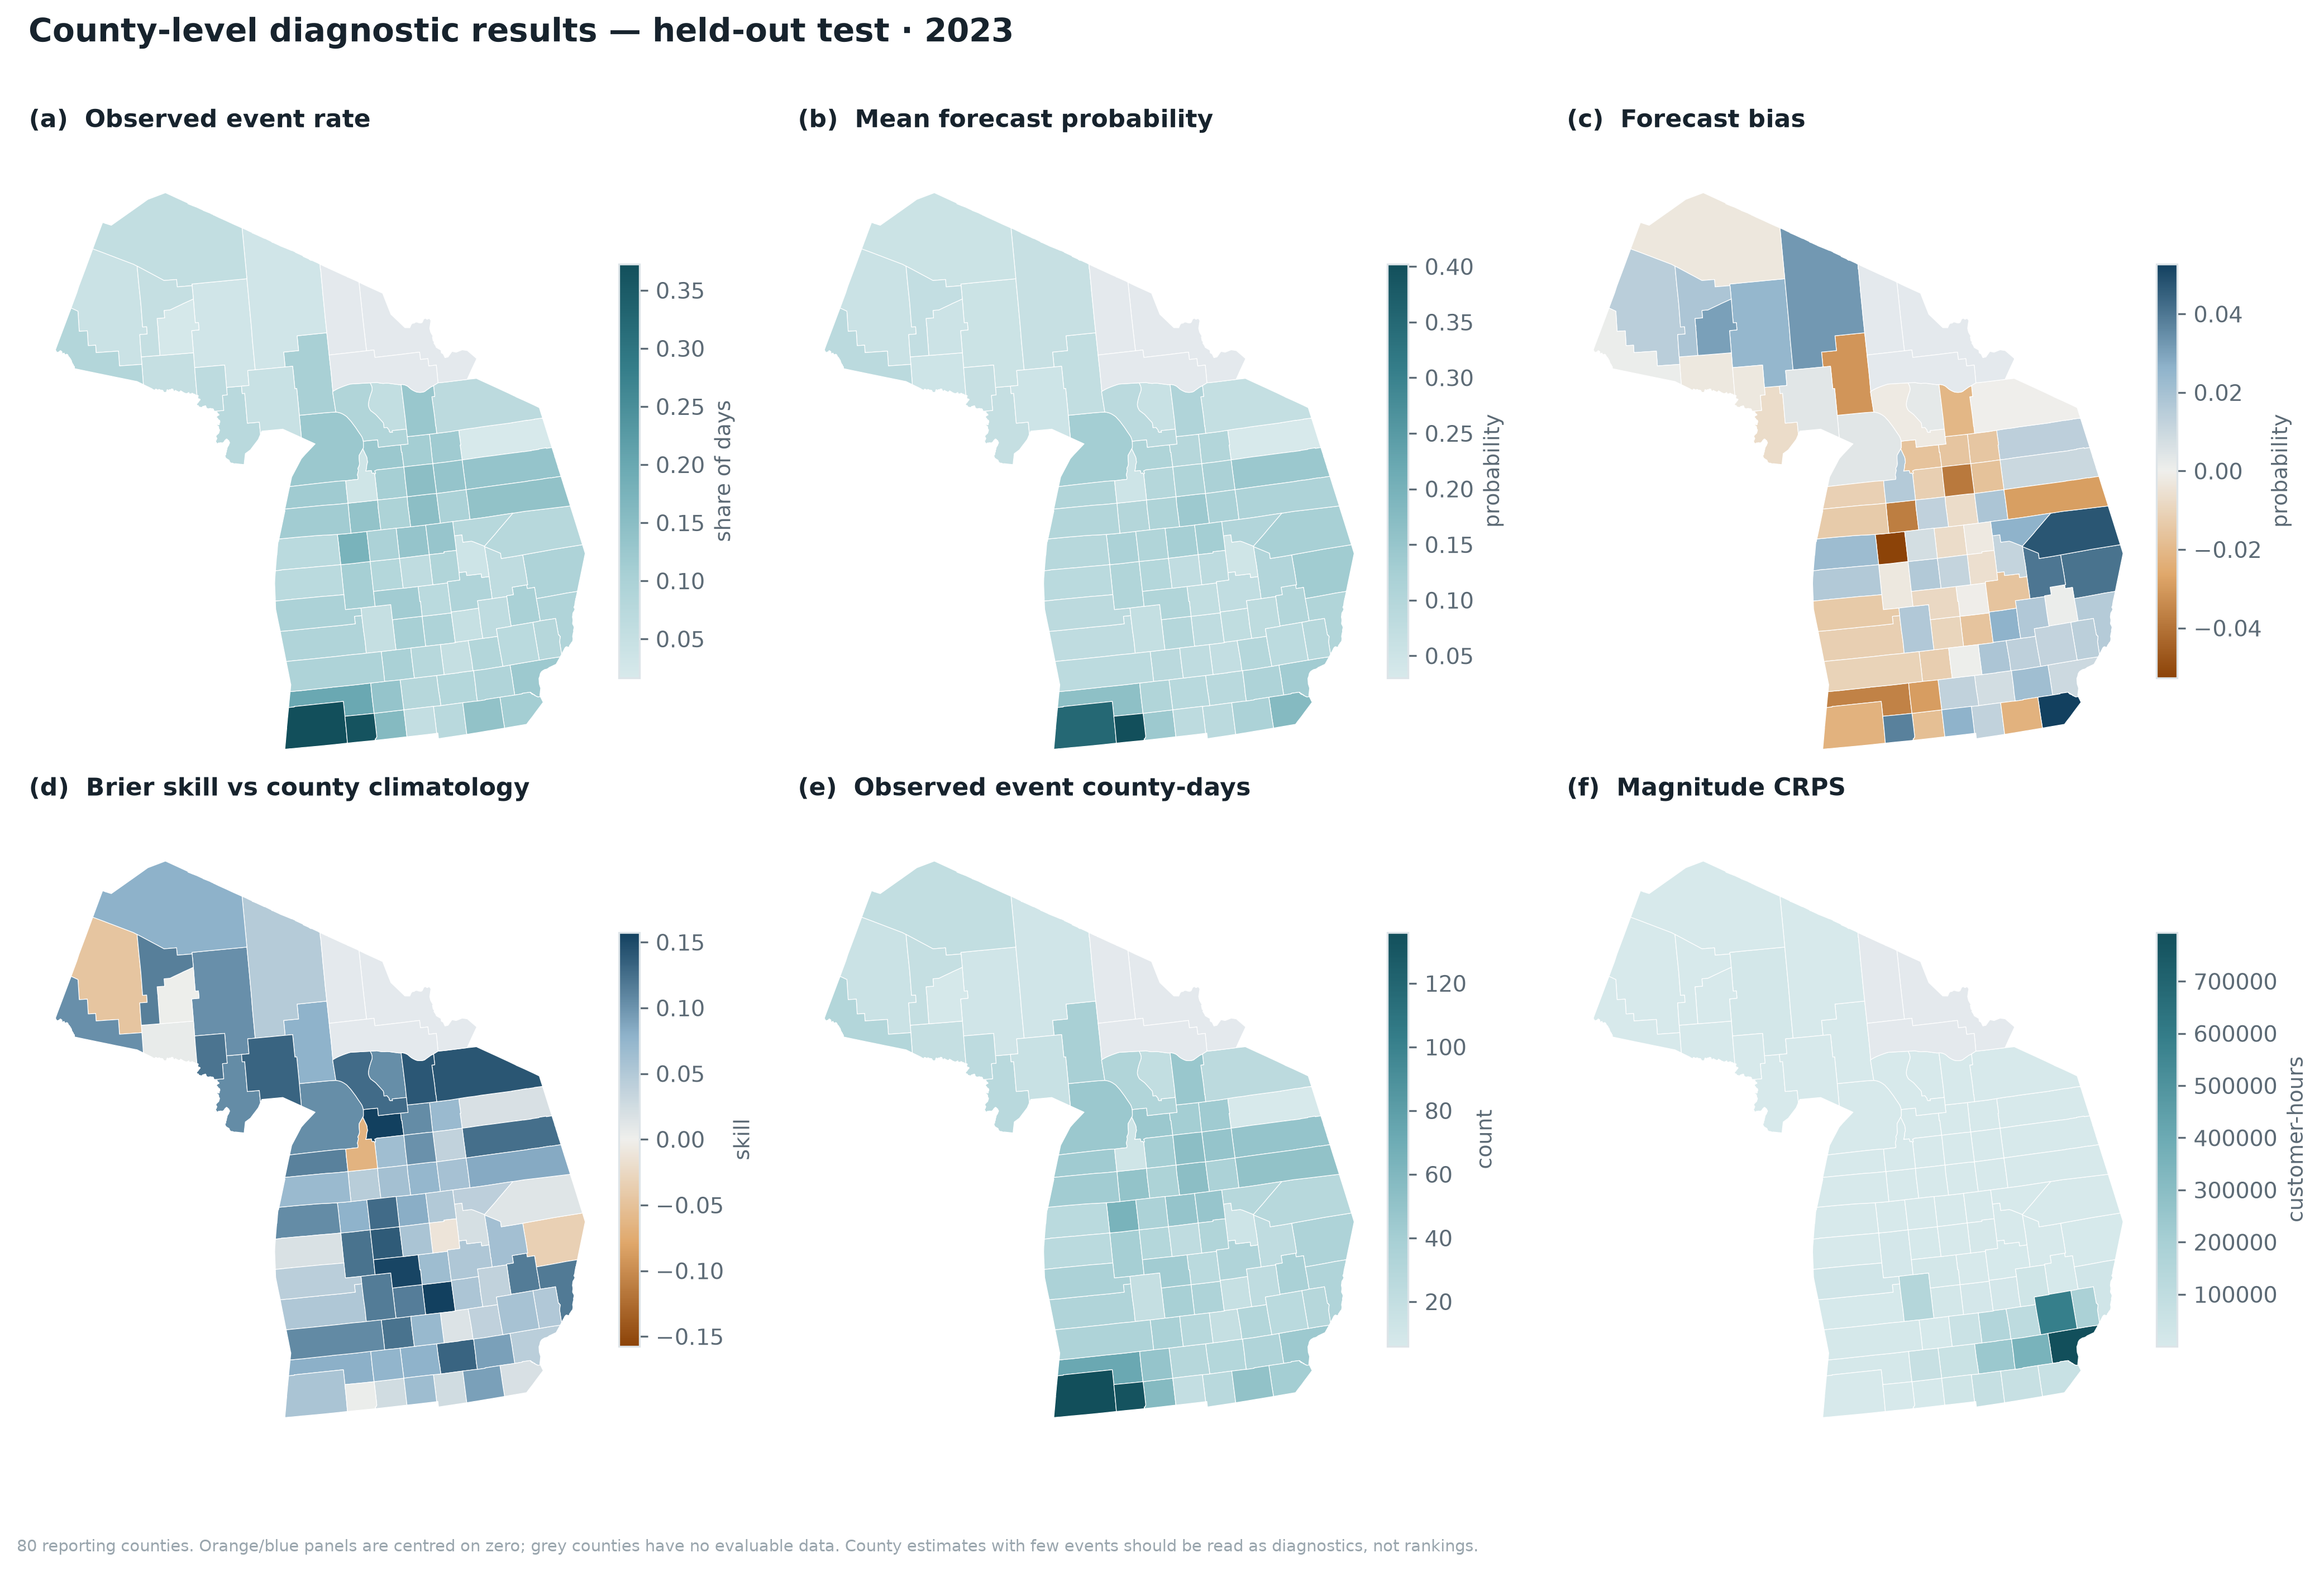
\includegraphics[width=0.95\textwidth]{../figures/phase2_county_diagnostics.png}
\caption{County-level diagnostics for the 2023 holdout: observed event rate,
mean forecast probability, bias, Brier skill against county climatology, event
count, and magnitude CRPS.}
\label{fig:county}
\end{figure*}

\subsection{GEFS case studies}

\begin{table*}[!tb]
\centering
\caption{Statewide \CH{} forecasts driven by GEFS for the two 2023 case
studies. Meteorological variance is the share of total predictive variance
attributable to spread among ensemble members, as opposed to the model's own
conditional uncertainty. These are operational case diagnostics and do not
replace the annual verification in Table~\ref{tab:verification}.}
\label{tab:gefs}
\small
\begin{tabular*}{\textwidth}{@{\extracolsep{\fill}}llrrrr@{}}
\toprule
\textbf{Case} & \textbf{Lead} & \textbf{Median} & \textbf{10--90\% interval} & \textbf{Observed} & \textbf{Met.\ variance} \\
\midrule
Aug 2023 wind event & day $-5$ & \num{53113} & \num{13677}--\num{364016} & \num{25577} & 9.6\% \\
Aug 2023 wind event & day $-3$ & \num{52981} & \num{14710}--\num{179218} & \num{25577} & 11.1\% \\
Aug 2023 wind event & day $-2$ & \num{76129} & \num{18787}--\num{433563} & \num{25577} & 26.8\% \\
Aug 2023 wind event & day $-1$ & \num{54824} & \num{14710}--\num{223482} & \num{25577} & 36.0\% \\
\addlinespace
Feb 2023 ice storm  & day $-5$ & \num{2454} & \num{0}--\num{15818} & \num{38402} & 11.5\% \\
Feb 2023 ice storm  & day $-3$ & \num{4272} & \num{0}--\num{20890} & \num{38402} & 18.1\% \\
Feb 2023 ice storm  & day $-2$ & \num{3184} & \num{0}--\num{14660} & \num{38402} & 9.0\% \\
Feb 2023 ice storm  & day $-1$ & \num{3462} & \num{0}--\num{16146} & \num{38402} & 6.7\% \\
\bottomrule
\end{tabular*}
\end{table*}

Each of the 31 GEFS members is bias-corrected against an ERA5 climatology built
from training and validation months only, passed through the feature pipeline,
and composed into 100 parametric draws, giving 3100 realizations per lead time.
The quantile mapping is fitted once per case and applied unchanged across all
leads; re-fitting it per lead forces every lead onto the same climatology and
erases exactly the lead-dependent dispersion the case studies are designed to
measure.

Table~\ref{tab:gefs} and Figure~\ref{fig:leads} report the results. The two
cases behave very differently. All four August wind-event intervals contained
the observation of $\num{25577}$ \CH{}, with medians roughly a factor of two
high and predictive intervals spanning an order of magnitude --- wide, but
honest. Every February ice-storm interval fell \emph{below} the observed
$\num{38402}$ \CH{}, at every lead. This is a genuine failure, not a wide
interval: the framework did not merely underpredict the ice storm, it assigned
the observed outcome negligible probability at all four lead times.

The variance decomposition adds a further caution. For the August case, the
share of predictive variance attributable to ensemble spread rises with
decreasing lead ($9.6\%$ at day $-5$ to $36.0\%$ at day $-1$), the expected
behaviour as the meteorological uncertainty becomes better resolved relative to
the model's fixed conditional uncertainty. For the February case the same share
stays between $6.7\%$ and $18.1\%$ with no monotone trend, consistent with a
hazard representation that is not responding to the ensemble information.

\begin{figure}[!tb]
\centering
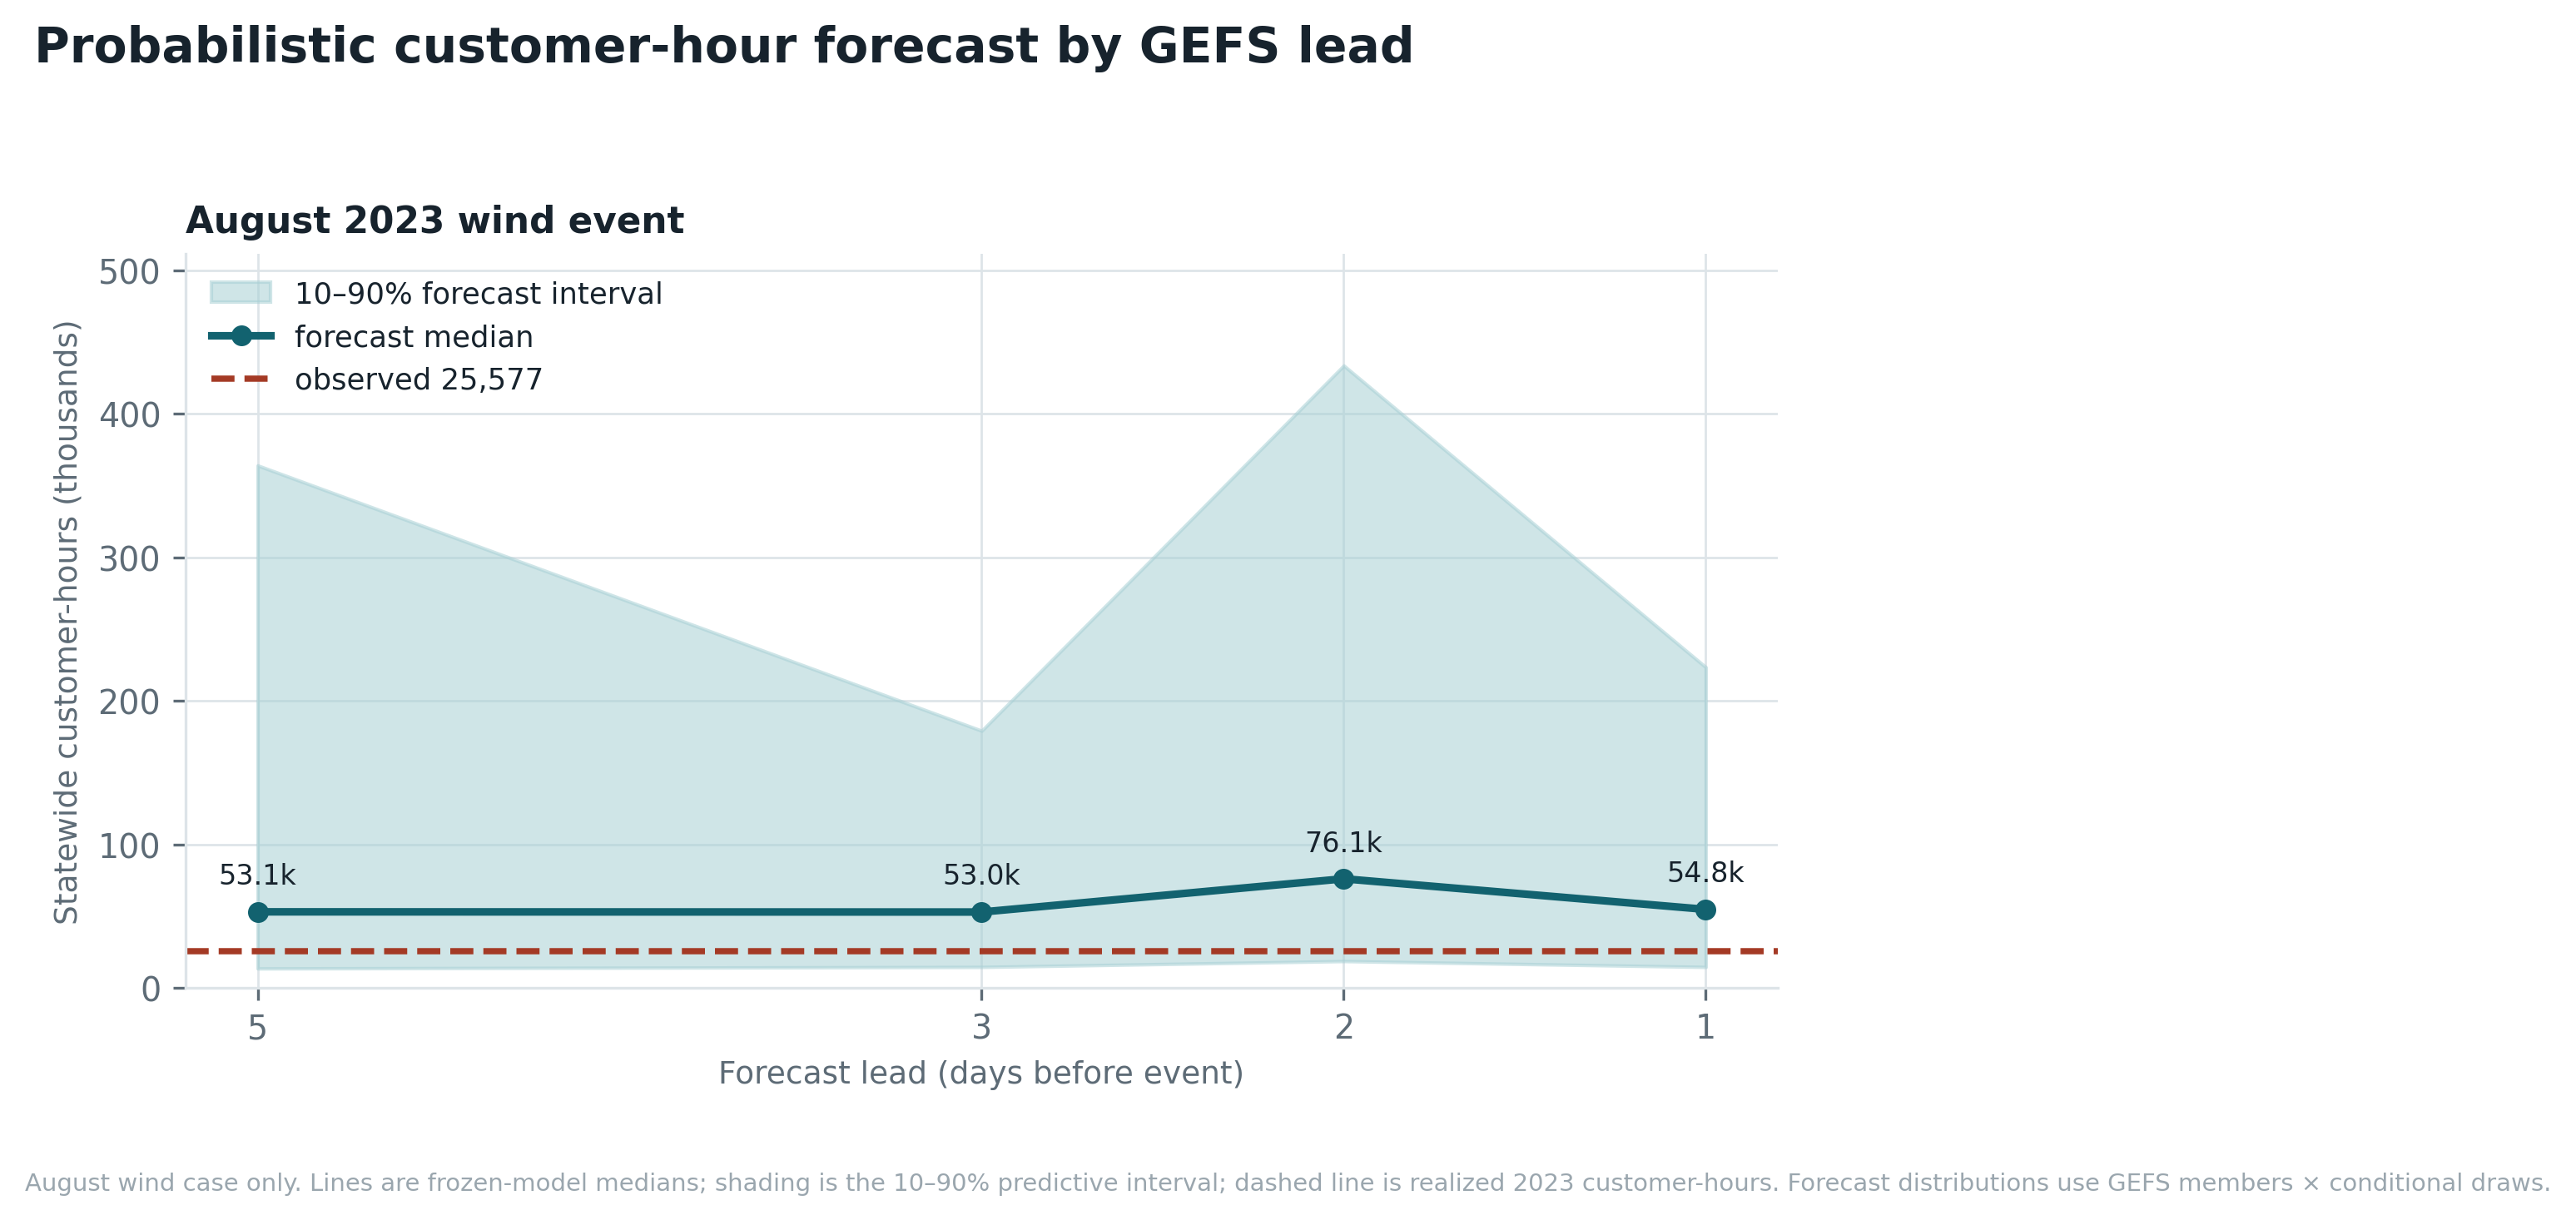
\includegraphics[width=\columnwidth]{../figures/phase2_gefs_lead_trajectories.pdf}
\caption{Statewide \CH{} forecasts for the August 2023 wind event by GEFS lead
time. Line: forecast median. Shading: 10--90\% predictive interval. Dashed line:
the $\num{25577}$ \CH{} observed.}
\label{fig:leads}
\end{figure}

% ============================================================================
\section{Decision value}\label{sec:value}
% ============================================================================

Skill is a property of forecasts; value is a property of decisions. We evaluate
value in two complementary ways: a dimensionless cost--loss analysis that
requires no monetary assumption, and a scenario analysis that does.

\subsection{Cost--loss framework}

In the standard cost--loss setting a decision maker can pay a protective cost
$C$ to avoid a loss $L$, and the optimal policy under a calibrated probability
forecast is to act when $p \ge C/L$
\citep{richardson2000value,zhu2002economicvalue}. Relative economic value
compares the expense of that policy against always acting on climatology and
against perfect information, and is dimensionless: it depends on the ratio
$C/L$, not on either quantity separately. Figure~\ref{fig:costloss} reports
relative value across the configured range $C/L \in [0.01, 0.50]$. This is the
part of the value analysis that stands on its own, because it introduces no
dollar figure at all.

\begin{figure}[!tb]
\centering
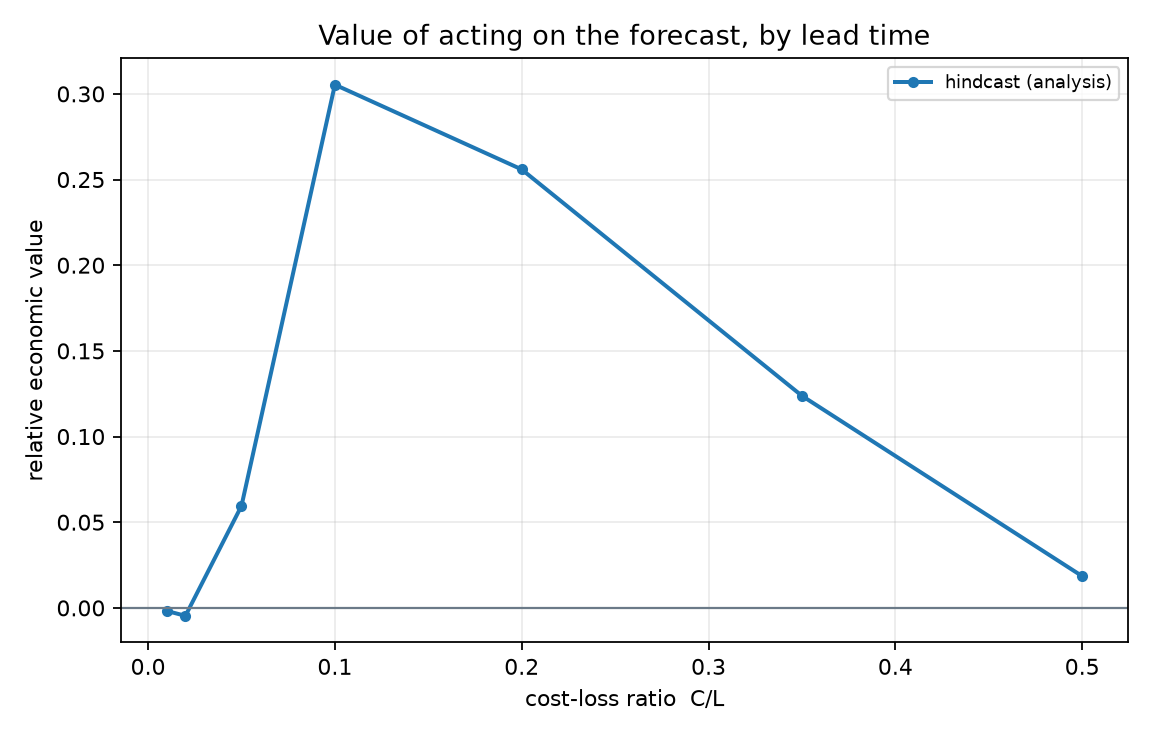
\includegraphics[width=\columnwidth]{../figures/phase2_cost_loss_value.png}
\caption{Relative economic value of the calibrated occurrence forecast across
cost--loss ratios, against climatology and perfect information.}
\label{fig:costloss}
\end{figure}

\subsection{Monetary scenarios and their standing}

\begin{notebox}
\small\textbf{Note on monetary figures.} The interruption-cost proxy below is a
\emph{documented placeholder}, constructed from a customer mix and per-hour
values in the configuration file, in the spirit of the ICE Calculator framework
\citep{sullivan2015ice}. It is not measured Michigan damage, repair expense, or
utility financial loss, and every avoided-cost figure is a counterfactual under
an assumed mitigation effectiveness, not an observed saving. These numbers
illustrate the arithmetic of the decision chain; they must be replaced with
region- and utility-specific inputs before any external economic claim.
\end{notebox}

The configured proxy is $\$25.12$ per customer-hour, from a mix of $88\%$
residential at $\$4.00$ and $12\%$ commercial at $\$180.00$ per customer-hour.
Applied to the $\num{126927110}$ \CH{} of interruption observed across the 2023
test year, that proxy corresponds to approximately $\$3.19$ billion --- a figure
whose only purpose here is to establish the scale at which even small
proportional reductions matter.

\subsection{Forecast-triggered action scenarios}

\begin{table*}[!tb]
\centering
\caption{Forecast-triggered action for the August 2023 wind event at a
cost--loss threshold of $C/L=0.10$ and an assumed $20\%$ consequence reduction.
Values are counterfactual potential impacts, not observed savings. February
ice-storm rows are omitted because no county crossed the trigger.}
\label{tab:impact}
\small
\begin{tabular*}{\textwidth}{@{\extracolsep{\fill}}lrrrr@{}}
\toprule
\textbf{Forecast lead} & \textbf{Counties triggered} & \textbf{Observed loss covered} & \textbf{Potential avoided \CH{}} & \textbf{Potential avoided cost proxy} \\
\midrule
$-5$ days & 52 / 80 & 99\% & \num{5057} & \$\num{127032} \\
$-3$ days & 45 / 80 & 95\% & \num{4874} & \$\num{122435} \\
$-2$ days & 50 / 80 & 99\% & \num{5057} & \$\num{127032} \\
$-1$ day  & 40 / 80 & 73\% & \num{3753} & \$\num{94270} \\
\bottomrule
\end{tabular*}
\end{table*}

To make the decision chain concrete, consider the August wind event at a
five-day lead. At each lead the model supplies a county probability $p_i$ and a
conditional \CH{} distribution. A county is flagged when $p_i \ge C/L = 0.10$;
at day $-5$, $52$ of the $80$ counties in the case cohort crossed that
threshold. Depending on lead time, the corresponding action package could
include pre-positioning crews and materials, requesting mutual aid, inspecting
vulnerable circuits, clearing vegetation, preparing switching plans, and
customer communication.

After the event, the trigger mask is compared against what was observed. Total
observed loss was $\num{25577}$ \CH{}; the triggered counties contained
$\num{25285}$ \CH{}, or $99\%$ of the event loss. Because no record of actual
interventions exists, the scenario assumes an action reduces realized
consequence by $20\%$:
\begin{align}
\text{avoided \CH{}} &= \num{25285} \times 0.20 = \num{5057},\\
\text{avoided proxy} &= \num{5057} \times \$25.12 \approx \$\num{127032}.
\end{align}

Table~\ref{tab:impact} repeats this across leads. Coverage is high and remarkably
flat from day $-5$ to day $-2$ ($99\%$, $95\%$, $99\%$) and falls at day $-1$ to
$73\%$ with fewer counties triggered. The non-monotonicity is itself worth
noting: for this event, a five-day forecast supported an action footprint at
least as useful as a one-day forecast, which is the operationally relevant
finding, since five days is where mutual aid and crew staging decisions are
actually made.

The counterfactual should not be over-read. The estimate says that had a
$20\%$-effective action been taken in the triggered counties, roughly
$\num{5057}$ \CH{} would have been avoided. It does not say that such an action
exists, that it costs less than its benefit, or that $20\%$ is the right
effectiveness. Establishing net benefit requires utility-specific action costs
and intervention outcome records, neither of which is public.

% ============================================================================
\section{Discussion}\label{sec:discussion}
% ============================================================================

\subsection{What the results support}

Three claims are supported by the frozen evaluation. First, weather-conditioned
county-day outage occurrence over Michigan is predictable with positive skill
against county climatology, and that skill survived a genuine one-shot holdout
(Brier skill $+0.075$ in 2023). Second, the conditional consequence
distribution carries positive skill against a climatological distribution
(CRPS skill $+0.084$), meaning the model conveys information about \emph{how
large} an event will be and not only whether one occurs. Third, the calibrated
probabilities are usable in a cost--loss decision rule, and in the August case
study the resulting trigger mask covered nearly all realized loss at
operationally useful lead times.

\subsection{The ice-storm failure}

The February ice storm is the most informative negative result in the study, and
it should not be filed as a wide interval. Every lead time placed the observed
consequence outside its 10--90\% interval, and the meteorological share of
predictive variance showed no lead-dependent structure. Two explanations are
consistent with the design and cannot be separated with the data at hand. The
freezing-rain predictor is a proxy --- precipitation accumulated within a
temperature band --- and does not resolve ice accretion, which depends on surface
and near-surface thermodynamic structure a $0.25^\circ$ field represents only
crudely. Alternatively or additionally, ice events are rare in the training
record, so the magnitude model has few analogues from which to learn the
appropriate conditional tail. Both point in the same direction: ice is the
regime where this framework is least trustworthy, and reporting it as such is
more useful than an aggregate score in which one rare regime is averaged away.

\subsection{Limitations}

\begin{description}[leftmargin=1.1em,itemsep=0.25em,topsep=0.3em]
\item[\textnormal{\emph{Spatial support of the target.}}] County aggregation
hides feeder topology, asset age, conductor type, vegetation-management
practice, and utility operations. A county is not a physical unit of the
distribution network, and no result here should be read as an asset-level
statement.

\item[\textnormal{\emph{Consequence without mechanism.}}] EAGLE-I records what
customers experienced, not why. The model can say that outage consequence is
likely; it cannot attribute that consequence to a cause.

\item[\textnormal{\emph{Hazard resolution.}}] ERA5 at $0.25^\circ$ under-resolves
convective gusts, and the freezing-rain and wet-snow terms are thermodynamic
proxies rather than accretion models.

\item[\textnormal{\emph{Case-study sample size.}}] Two case studies cannot
characterize forecast performance. The GEFS bias correction is fitted on a small
sample, and the case results are diagnostics, not verification.

\item[\textnormal{\emph{Restoration.}}] The duration model did not beat county
persistence on median absolute error in 2023. Restoration is an operations
problem more than a meteorological one.

\item[\textnormal{\emph{Economics.}}] All monetary figures rest on placeholder
interruption costs and an assumed mitigation effectiveness, and the asset-count
denominator behind any per-asset break-even figure is a customer-count ratio,
not a pole and span inventory.
\end{description}

\subsection{Future work}

The most valuable additions are not more model capacity but better data:
utility-specific interruption costs and intervention records would convert the
counterfactual scenarios into measured value; feeder-level outage records would
allow the target to be defined on a physical unit of the network; and a
higher-resolution or convection-permitting hazard representation would address
the gust and ice-accretion limitations directly. On the modelling side, the
regime-stratified results suggest that a hazard-specific treatment of ice, with
an explicit accretion formulation, would address the study's clearest failure
mode more effectively than a general increase in model flexibility.

% ============================================================================
\section{Conclusions}
% ============================================================================

We have presented a county-day probabilistic framework linking reanalysis and
ensemble forecasts to distribution-system outage consequence over Michigan, and
evaluated it under a frozen split scored once on a full held-out year. The
occurrence model beats county climatology, a reduced logistic GLM, and a
gust-threshold rule on the 2023 holdout; the conditional magnitude distribution
carries positive skill against climatology; and the calibrated probabilities
support a cost--loss decision rule whose trigger mask covered $99\%$ of realized
loss at a five-day lead in the August case study. Equally, the framework did not
beat county persistence for restoration duration, and it failed on the February
ice storm at every lead time. Reporting both outcomes from a single frozen
evaluation is the point of the design: the framework is useful for wind-driven
outage anticipation at operational lead times, and it is not yet reliable for
ice.

% ============================================================================
\section*{Data availability}
% ============================================================================

EAGLE-I outage records are distributed by Oak Ridge National Laboratory
\citep{brelsford2024eaglei} via figshare
(\href{https://doi.org/10.6084/m9.figshare.24237376}{10.6084/m9.figshare.24237376}).
ERA5 is available from the Copernicus Climate Data Store and the ECMWF ARCO
archive. GEFS is available from the NOAA public cloud archive. NLCD percent tree
canopy cover is distributed by the Multi-Resolution Land Characteristics
Consortium. County geometry is from U.S.\ Census TIGER/Line.

\section*{Code availability}

The complete analysis pipeline, configuration, and reporting code are available
at
\href{https://github.com/afahadabdullah/storm-outage-risk-mi}{github.com/afahadabdullah/storm-outage-risk-mi}.
The study region, temporal splits, event definition, and hazard thresholds are
set in a single configuration file, so the framework can be moved to another
region without modifying analysis code.

\section*{Competing interests}

The author declares no competing interests.

% ============================================================================
\bibliographystyle{plainnat}
\bibliography{refs}

% ============================================================================
\clearpage
\onecolumn
\appendix
\section{Supplementary figures}\label{app:figs}
% ============================================================================

\begin{figure}[!h]
\centering
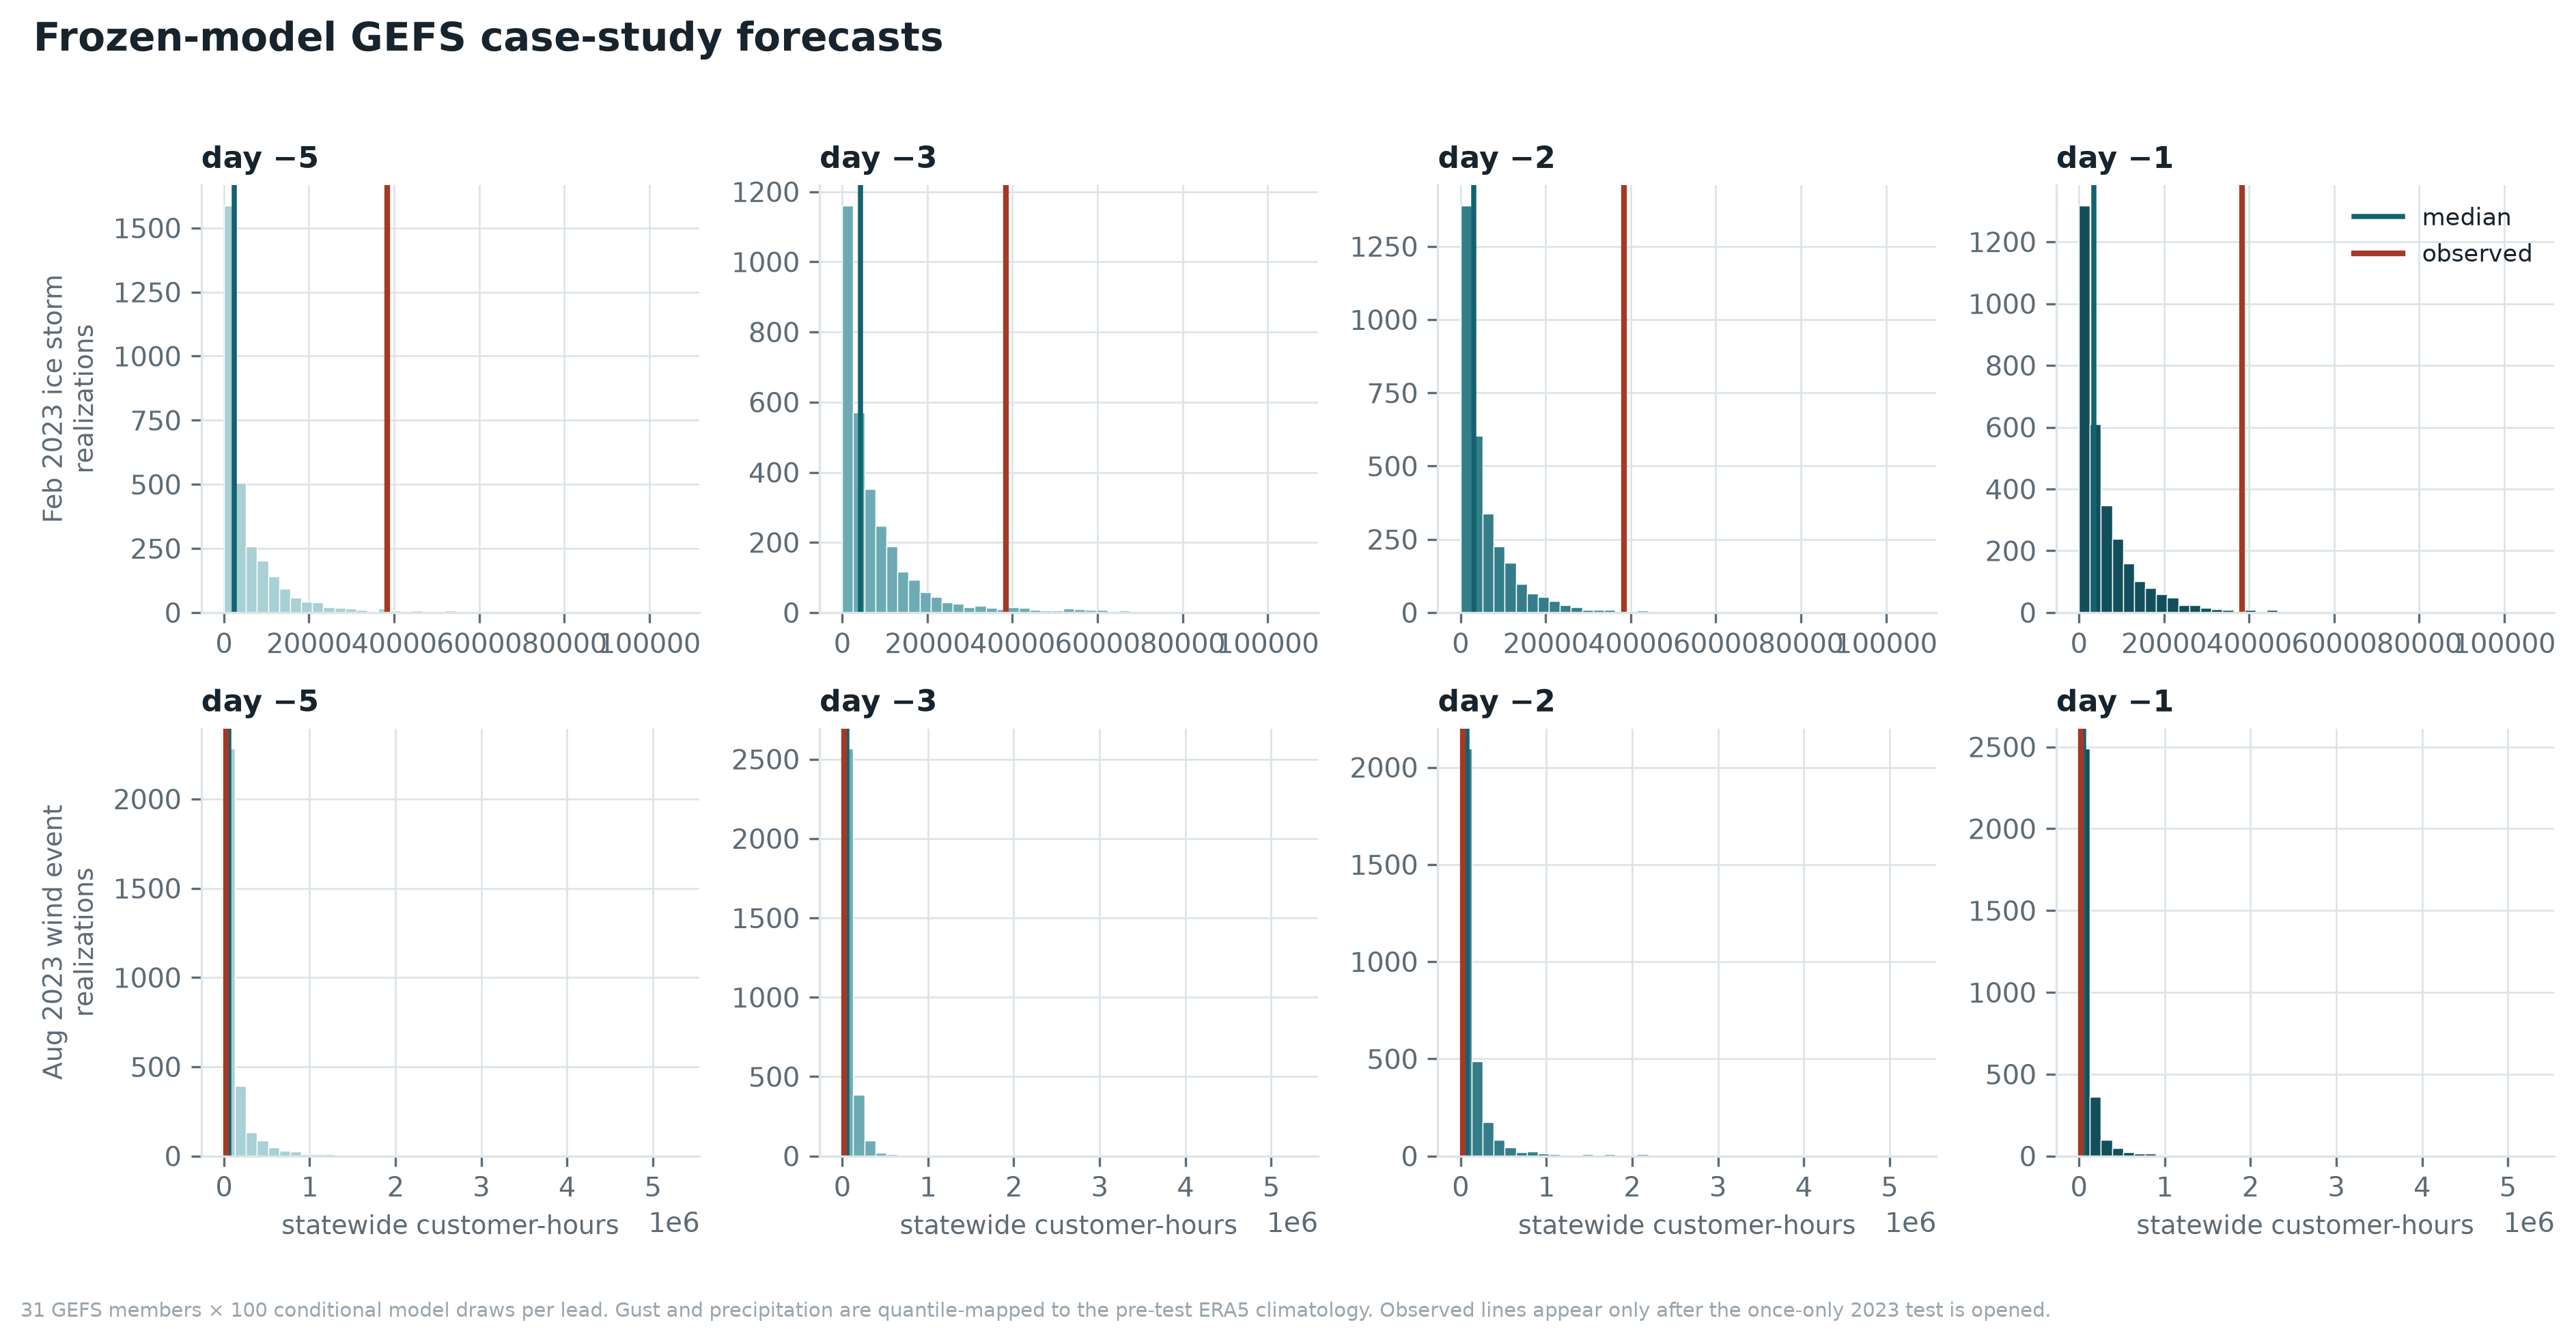
\includegraphics[width=0.86\textwidth]{../figures/phase2_gefs_case_studies.png}
\caption{GEFS-driven predictive distributions of statewide \CH{} for both 2023
case studies at all four lead times. The August wind event (contained at every
lead) and the February ice storm (below the observation at every lead) are shown
on comparable axes.}
\label{fig:appcases}
\end{figure}

\begin{figure}[!h]
\centering
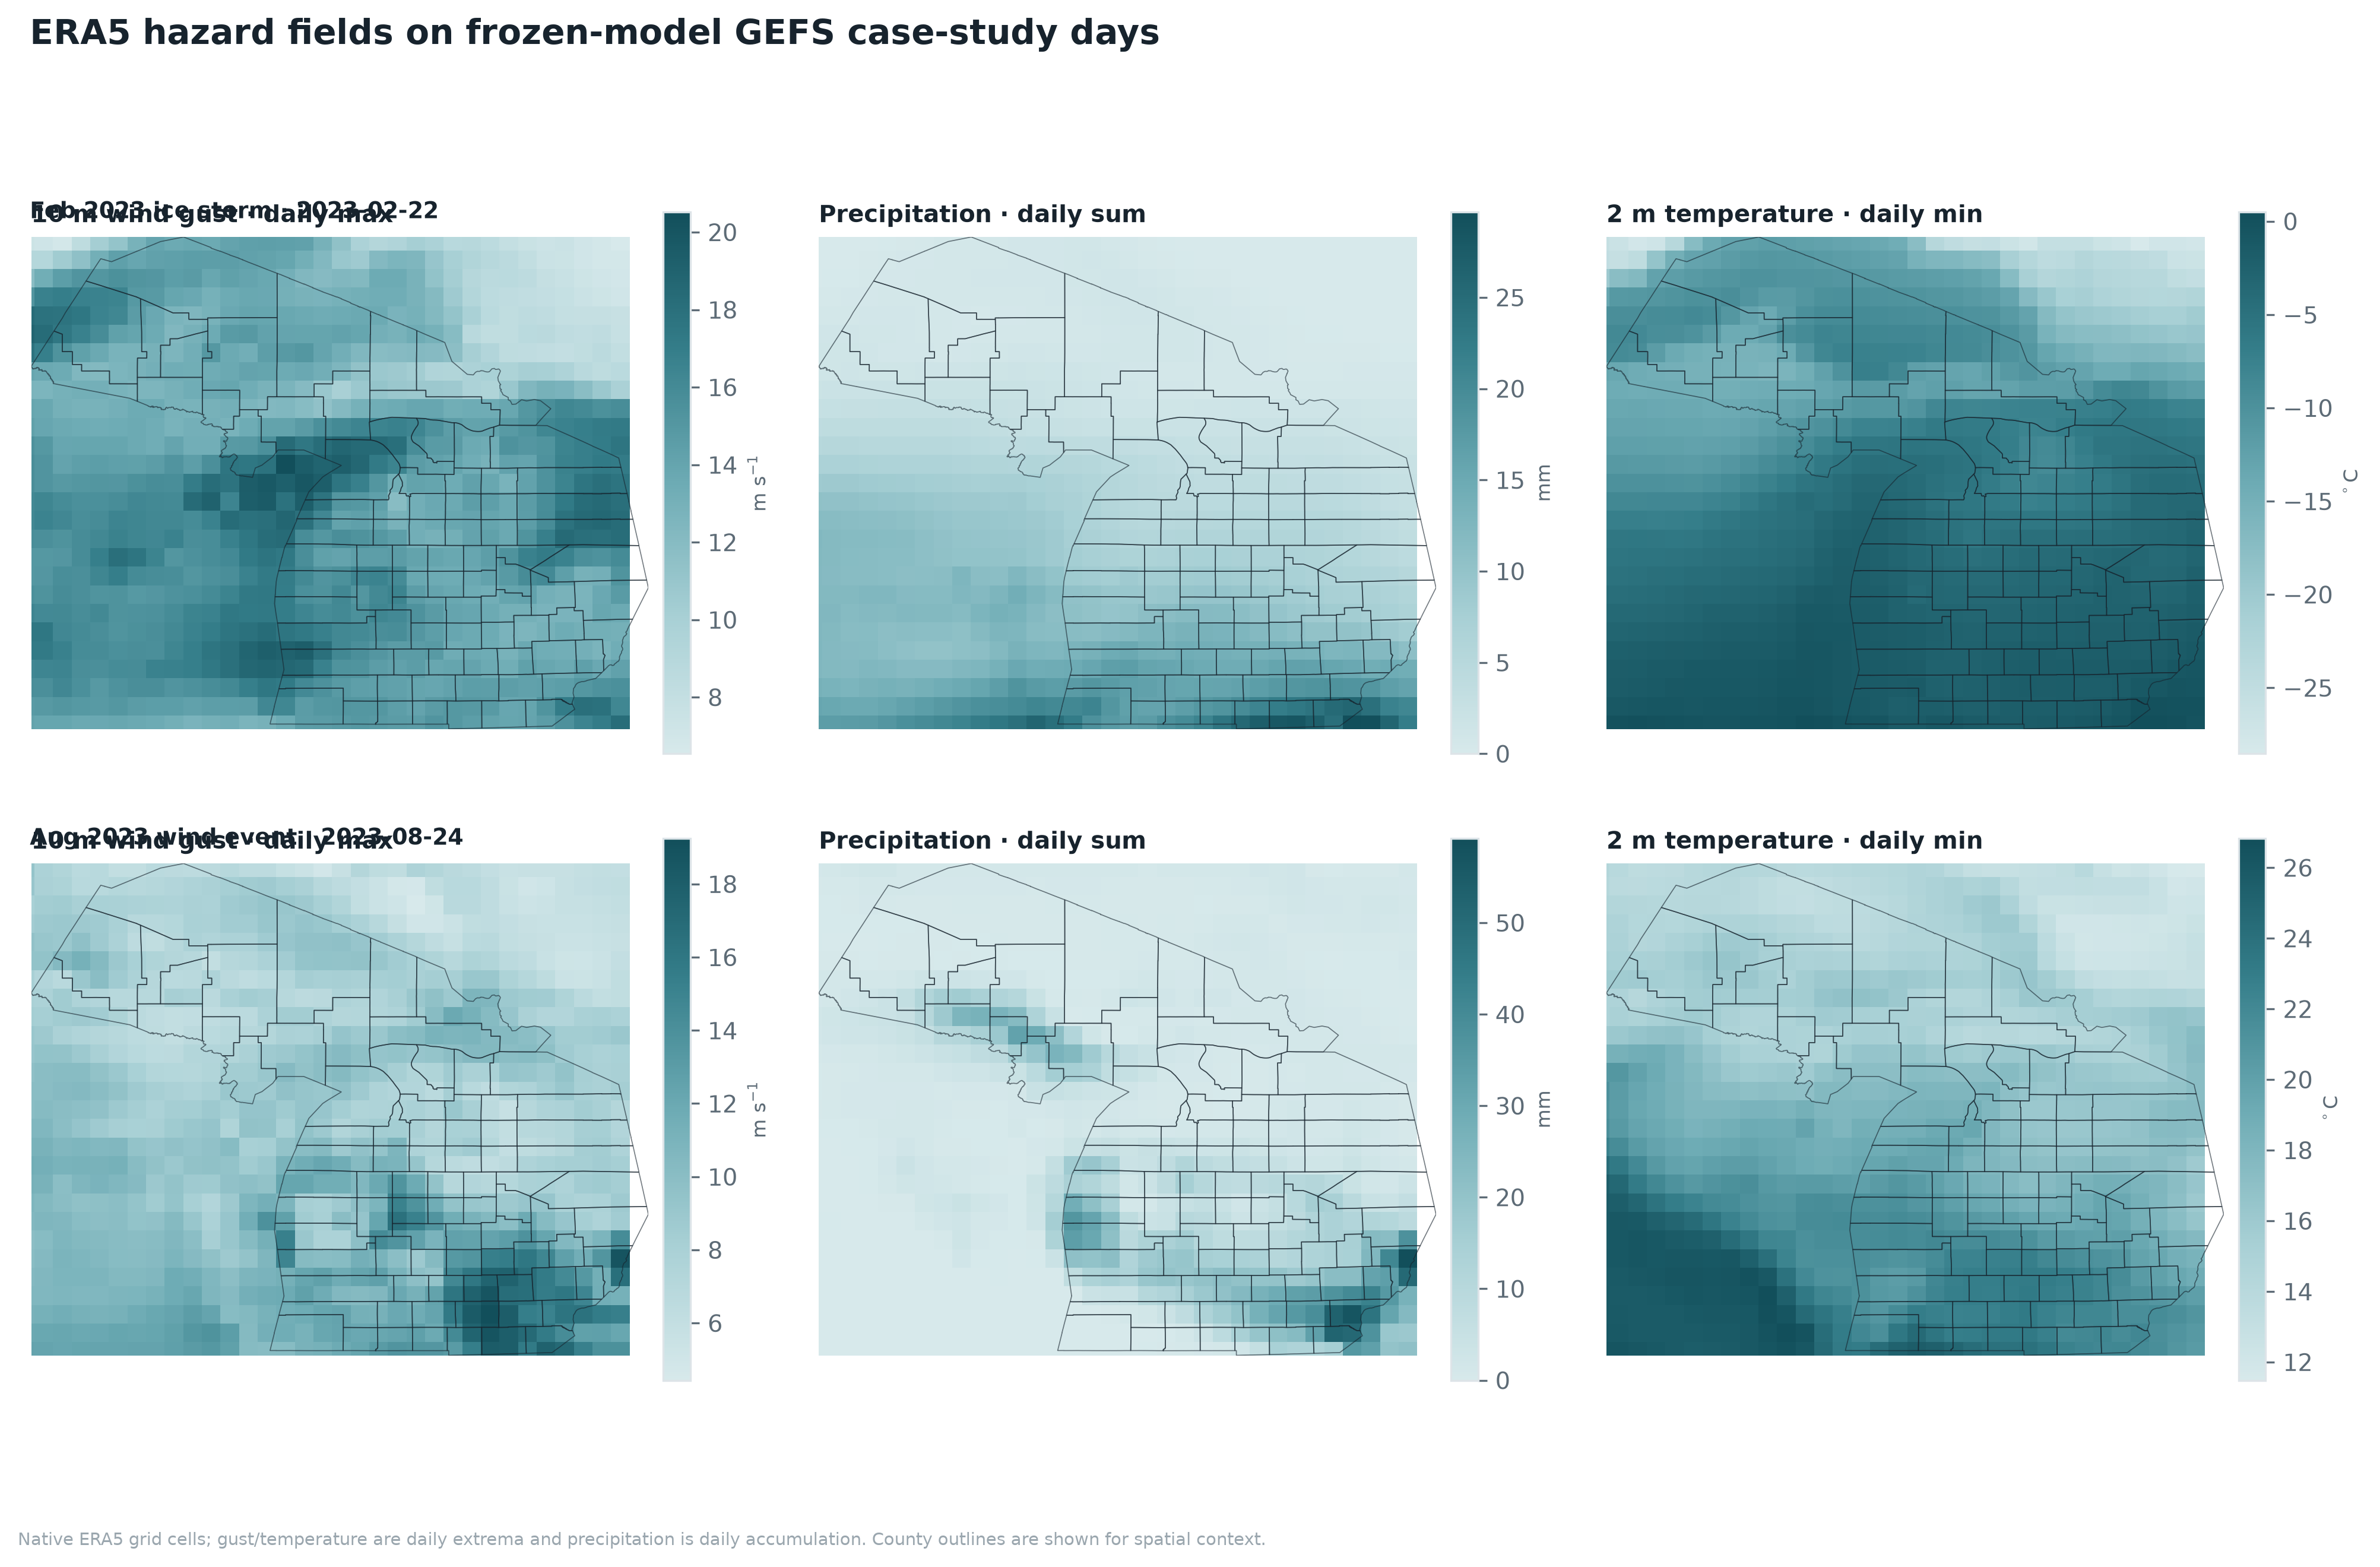
\includegraphics[width=0.86\textwidth]{../figures/phase2_case_hazards.png}
\caption{ERA5 hazard fields on the two case-study days, showing the
meteorological setting the model conditioned on in each case.}
\label{fig:apphazards}
\end{figure}

\begin{figure}[!h]
\centering
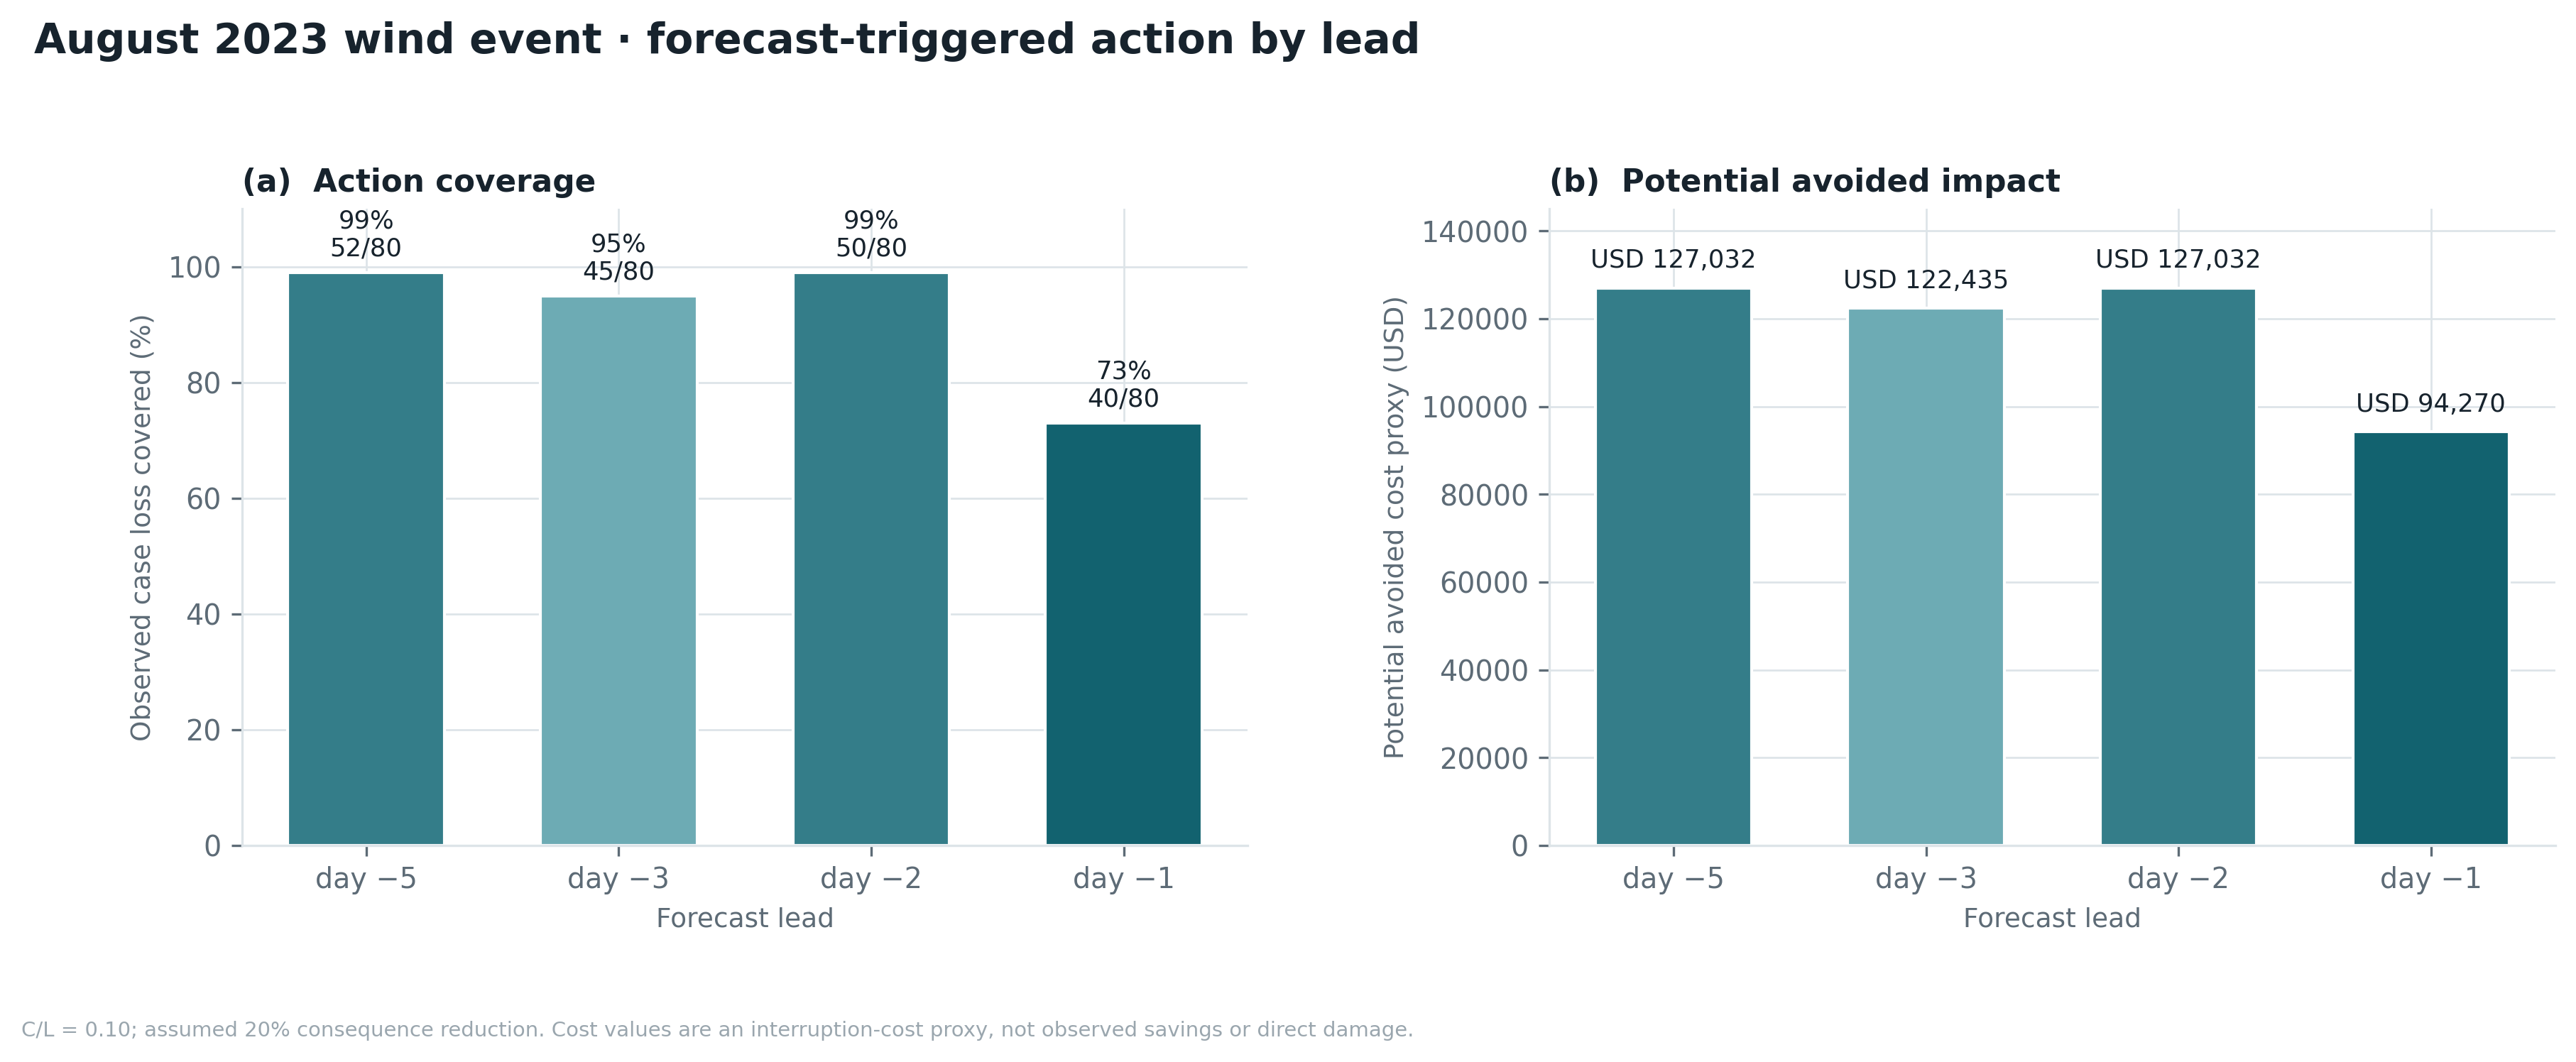
\includegraphics[width=0.78\textwidth]{../figures/phase2_forecast_triggered_impact_by_lead.pdf}
\caption{Forecast-triggered action for the August 2023 wind event by lead time:
share of observed loss contained within triggered counties, and the potential
avoided interruption-cost proxy under the $20\%$ mitigation assumption. Labels
above the coverage bars give triggered counties out of 80. All monetary values
are placeholders as described in Section~\ref{sec:value}.}
\label{fig:appimpact}
\end{figure}

\end{document}
